\section{Zadanie 11}
(igła Buffona)
Płaszczyznę przecięto zbiorem poziomych linii. Odstęp między dwoma
sąsiednimi liniamy wynosi \(d\). Rzucamy igłą długości \(l\) na tę
płaszczyznę. Wyznacz prawdopodobieństwo przecięcia linii.
\subsection*{Rozwiązanie}
Rozważymy dwa przypadki
\subsubsection*{Igła krótsza (lub równa) od dystansu między liniami}
Mamy \(l \leq d\). Jeśli igła po rzuceniu utworzy z liniami 
jakiś kąt ostry \(\alpha\), to przetnie się z taką linią, której
odległość od środka igły była co najwyżej
\(\frac{l}{2}\cdot\sin \alpha\).
\begin{center}
  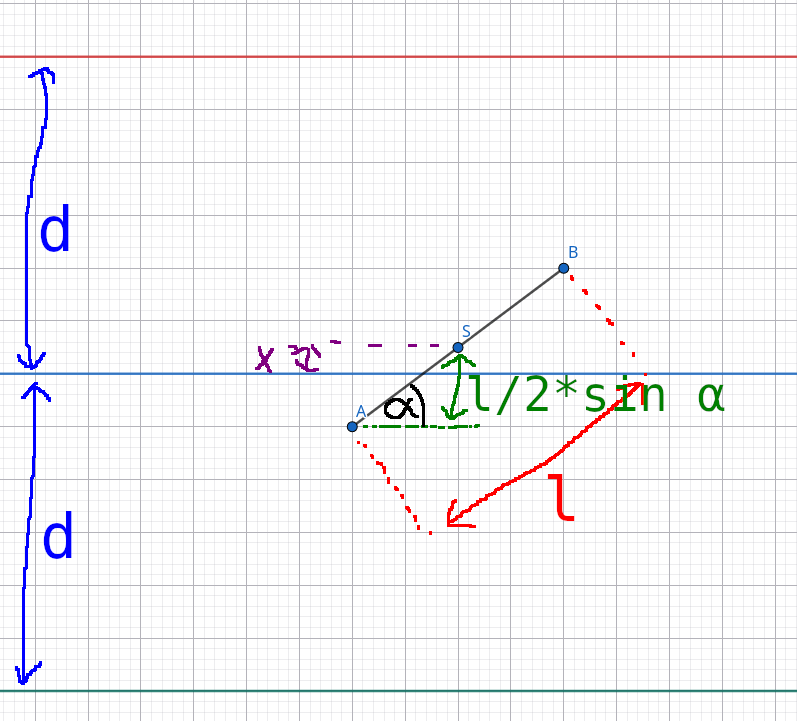
\includegraphics[width=0.7\textwidth]{tasks/11-1.png}
\end{center}

Zdarzenie jest cykliczne, więc możemy założyć że
\(\alpha \in \big[0, \frac{\pi}{2}\big]\).
\(\alpha\) ma rozkład jednostajny.

Odległość \(X\) środka igły od najbliższej linii przyjmuje wartości z przedziału
\(\big[0, \frac{d}{2}\big]\). Ma rozkład jednostajny.

\[
    P(\text{sukces})
    = P\left(\frac{l}{2}\sin \alpha \geq X\right)
    = \int_0^{\frac{\pi}2} \frac{2}{\pi} 
    \cdot \left(\frac{l}{2}\sin \alpha \right) \cdot 
    \frac{2}{d}~d\alpha
\]
Gdzie rozbiliśmy zdarzenie na podzdarzenia: \(X\) większy od już
ustalonego \(\alpha\)
\begin{itemize}
    \item \(\frac{2}{\pi}\) --- gęstość rozkładu \(\alpha\) (jednostajna)
    \item \(\frac{l}{2}\sin \alpha\) --- "ilość" takich \(X\)-ów, które
    spełniają nierówność
    \item \(\frac{2}{d}\) --- gęstość zmiennej \(X\) (jednostajna)
\end{itemize}
W prezentacji https://probabil.tcs.uj.edu.pl/docs/igla.pdf
jest przedstawione to samo za pomocą całki podwójnej, tutaj został
pominięty ten krok.

\[
    P(\text{sukces})
    = \frac{2l}{\pi d} \int_0^{\frac{\pi}2} \sin \alpha
    = \frac{2l}{\pi d}~(-\cos\alpha) \Big|_{0}^{\frac{\pi}{2}}
    = \frac{2l}{\pi d} \cdot 1
    = \frac{2l}{\pi d}
\]

\subsubsection*{Igła dłuższa od dystansu między liniami}
Mamy \(l > d\). Po ustaleniu jakiejś \(\alpha\), mieliśmy
\(
P(X \leq \frac{l}{2}\sin\alpha) = 
\frac{l}{2}\sin \alpha \cdot \frac{2}{d}
\).

Teraz nie jest to już prawdą. Może się zdarzyć, że dla jakiejś
\(\alpha\), nie jest możliwe wylosowanie \(X\) który nie spełni nierówności.

Na przykład, dla \(\alpha = \frac{\pi}{2}\).
Igła jest pionowo i jest dłuższa niż dystans między liniami,
więc na pewno którąś przetnie. Według naszego naiwnego wzorku
ma na to prawdopobieństwo \(\frac{l}{d} > 1\).

Dopóki \(\frac{l}{d}\sin \alpha\) nie przekracza 1 wszystko działa. Można
więc policzyć:

\[
    P(\text{sukces})
    = P\left(\frac{l}{2}\sin \alpha \geq X\right)
    = \int_0^{\frac{\pi}2} \frac{2}{\pi} 
    \cdot
    \max\left(1,~\frac{l}{2}\sin \alpha \frac{2}{d}
    \right)
    ~d\alpha
\]

Mamy \(\frac{l}{d}\sin\alpha > 1\) wtw. \(\alpha > \arcsin \frac{d}{l}\).
Można więc łatwo rozbić na sumę dwóch całek

\[
    \frac{2}{\pi} \int_0^{\frac{\pi}2} 
    \max\left(1,~\frac{l}{d}\sin \alpha \right)
    ~d\alpha
    = \frac{2}{\pi} \left(
    \int_0^{\arcsin\frac{d}{l}} \frac{l}{d}\sin \alpha
    +
    \int_{\arcsin\frac{d}{l}}^{\frac{\pi}{2}} d\alpha
    \right)
\]
\[
    = \frac{2}{\pi} \left(
    \frac{l}{d}~(-\cos\alpha) \Big|_{0}^{\arcsin\frac{d}{l}}
    + \left(\frac{\pi}{2} - \arcsin\frac{d}{l} \right)
    \right)
\]
\[
    = \frac{2}{\pi} \left(
    \frac{l}{d}\left(1 - \cos\left(\arcsin\left(\frac{d}{l}
    \right)\right)\right)
    + \left(\frac{\pi}{2} - \arcsin\frac{d}{l} \right)
    \right)
\]
\[
    \frac{2l}{\pi d} \left(
    1 - \sqrt{1 - \left(\frac{d}{l}\right)^2}\right)
    + \frac{2}{\pi}\arccos\frac{d}{l}
\]

\subsection*{Odpowiedź}
\[
\boxed{
\frac{2l}{\pi d}\text{, gdy } l \leq d
}
\]
\[
\boxed{
    \frac{2l}{\pi d} \left(
    1 - \sqrt{1 - \left(\frac{d}{l}\right)^2}\right)
    + \frac{2}{\pi}\arccos\frac{d}{l}
    \text{, gdy } l > d
}
\]
